\section{Game library}

\begin{frame}{2D games}
	\begin{itemize}
		\item 2D game library implemented by Malte Sehmer (bachelor thesis)
		\item Supports sprites (loaded from bitmap files) and animations
		\item Collision detection based on rectangle colliders (polygon colliders are conceptually implemented)
		\item Linear and accelerated movements are implemented (e.g. gravity)
		\item Particle system (bachelor thesis by Abdulbasir Gümüs)
	\end{itemize}
	\begin{minipage}{0.49\textwidth}
		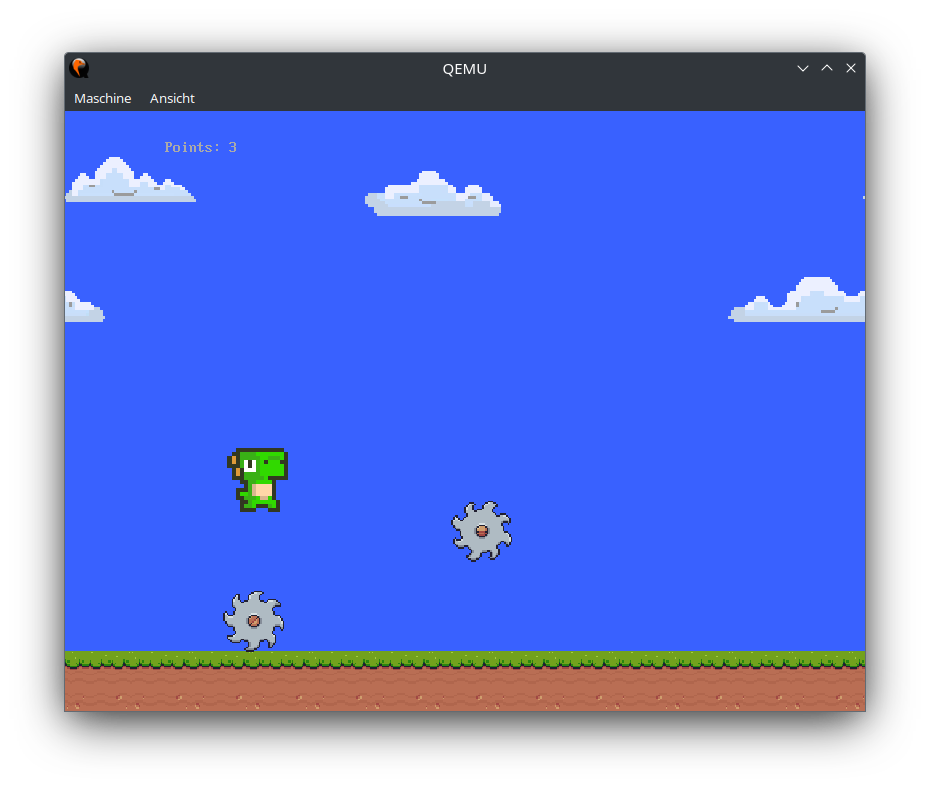
\includegraphics[width=0.9\textwidth]{img/dino}
	\end{minipage}
	\begin{minipage}{0.49\textwidth}
	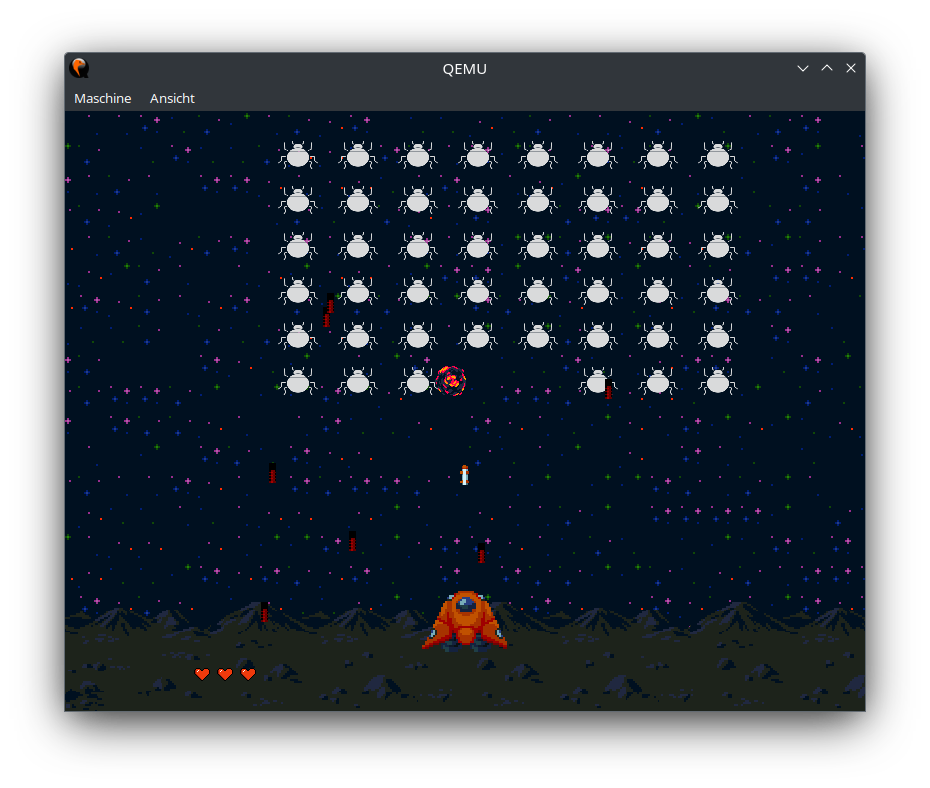
\includegraphics[width=0.9\textwidth]{img/bug}
	\end{minipage}
	\pause
	\begin{center}
		\textbf{But can it run Crysis?}
	\end{center}
\end{frame}

\begin{frame}{3D games - Work in Progress}
	\begin{itemize}
		\item 3D extension to the game library (bachelor thesis by Richard Schweitzer)
		\item Supports wireframe 3D-objects loaded from OBJ files
		\item Collision detection based on spheres
		\item Many features are missing (e.g. texturing, z-buffering, etc.)
	\end{itemize}
	\begin{minipage}{0.49\textwidth}
		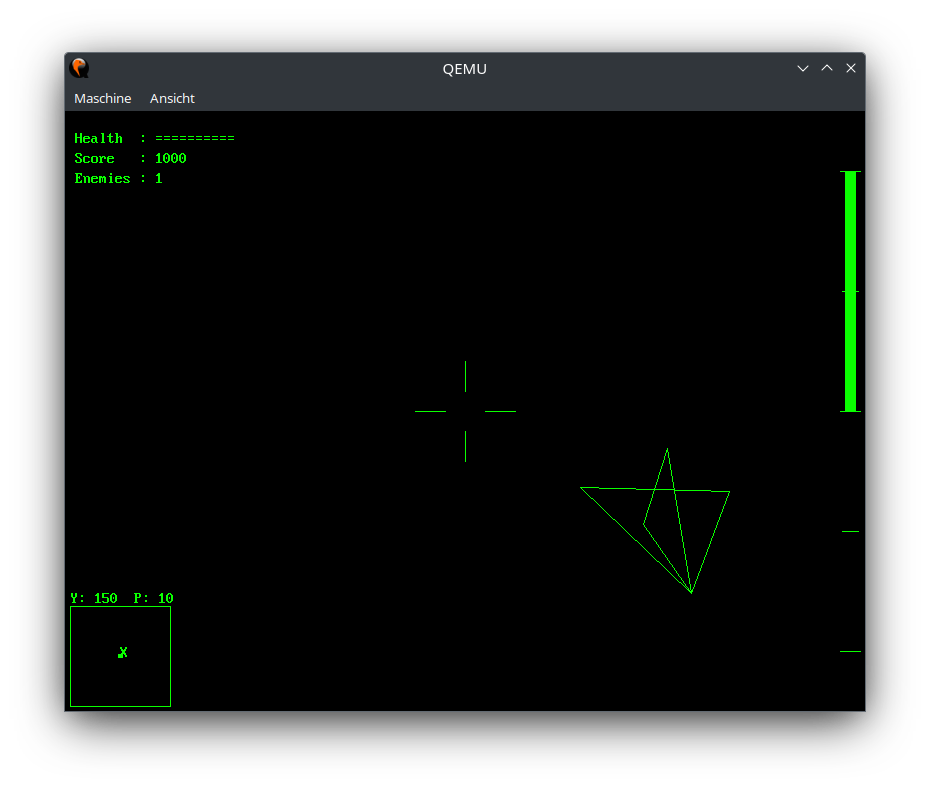
\includegraphics[width=0.95\textwidth]{img/battlezone1}
	\end{minipage}
	\begin{minipage}{0.49\textwidth}
		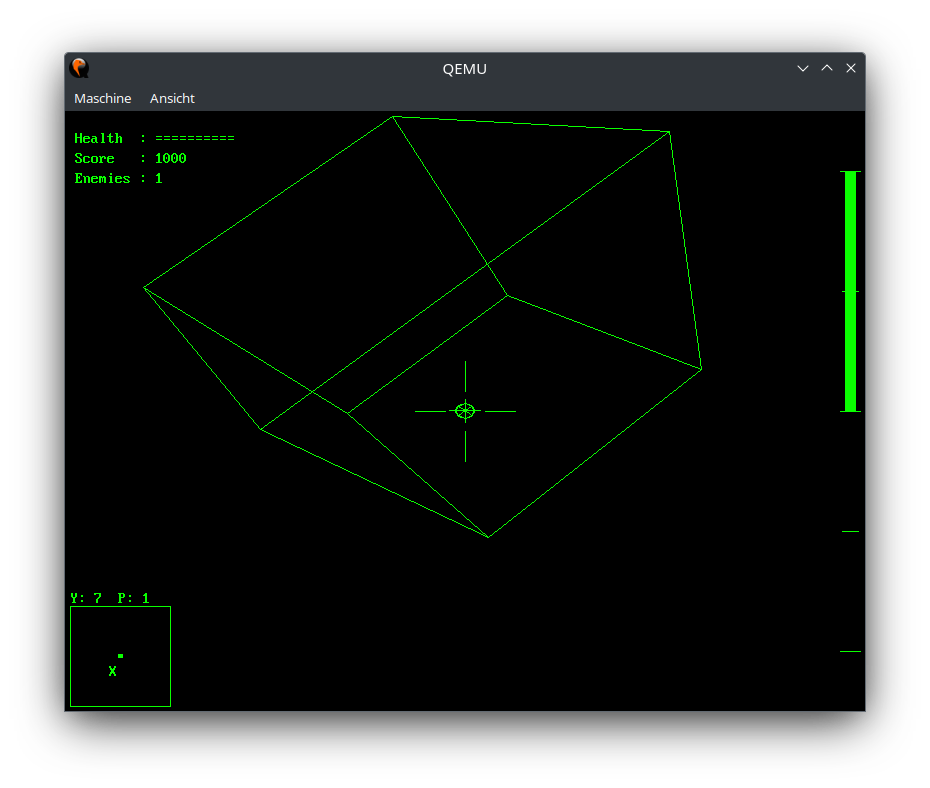
\includegraphics[width=0.95\textwidth]{img/battlezone2}
	\end{minipage}
\end{frame}
